
\subsubsection{Problem}
\textcolor{red}{$[$ insert continuous equations here $]$}

\subsubsection{Numerical scheme}
We compute a numerical approximation of \textcolor{red}{insert ref of continuous equations} on a Cartesian grid using the Yee scheme. Let $n$ denote the time step, as usual $t_n = n \Delta t$. $H_z$ will then be taken on a half time step, and our equation, discretized in them write :
 \textcolor{red}{$[$ insert time-discretized equations here $]$}
 We discretize our equation on staggered grid, meaning $E_x$, $u_x$, $E_y$, $u_y$ and $H_z$ are not and the same grid. Evidently we already stated it for $H_z$ in the time discretization. Fig.~\ref{schemepos} shows the positions of $Ex$, $u_x$ (black dots), $E_y$ $u_y$ (blue dots) and $H_z$ (red dots) on the discretized grid in space and time. We obtain the following discretized equations, 

\be 
\eps_0 \frac{E_x\inp- E_x\midin}{\Delta t} = -e N_e \frac{u_x\inp + u_x \midin}{2},
\label{eq:ns1}
\ee 
\be
\eps_0 \frac{E_y\ihnp-E_y\ihn}{\Delta t}+ \frac{H_z\ipnh-H_z\inh}{\Delta x} = -eN_x \frac{u_y\ihnp + u_y\ihn}{2} ,
\label{eq:ns2}
\ee
\be
 \frac{H_z\inh-H_z\inmh}{\Delta t}+ \frac{E_y\ihn-E_y\imhn}{\Delta x}=0,
 \label{eq:ns3}
\ee
\be 
m_e \frac{u_x\inp-u_x\midin }{\Delta x} = e N_e \frac{E_x\inp+E_x\midin}{2}-\nu m_e\frac{u_x\inp+u_x \midin}{2}+ eB_0\frac{u_y\ihn+u_y\ihnp}{2},
\label{eq:ns4}
\ee
\be
m_e \frac{u_y\ihnp-u_y\ihn}{\Delta t} = eN_e \frac{E_y\ihnp + E_y\ihn}{2}- \nu m_e \frac{u_y\ihnp +u_y\ihn}{2}-eB_0 \frac{u_x\midin+u_x\inp}{2},
\ee
\begin{figure}[H]
	\begin{center}
		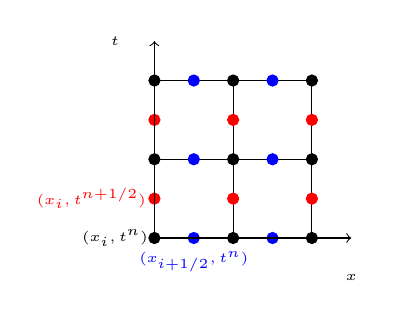
\begin{tikzpicture}

\draw (0, 0) grid (2, 2);
\foreach \x in {0,1,2}
	\foreach \y in {0,1,2}
		\draw[fill](\x,\y) circle (2pt) ;
\foreach \x in {0.5,1.5}
	\foreach \y in {0,1,2}
		\draw[fill,blue](\x,\y) circle (2pt) ;
\foreach \x in {0,1,2}
	\foreach \y in {0.5,1.5}
		\draw[fill,red](\x,\y) circle (2pt) ;		
 \draw[->] (0,0) -- (0,2.5);
  \draw[->] (0,0) -- (2.5,0);
      \coordinate (Origin)   at (0,0);
      \node (xlab) at (2.5,-0.5){\tiny $x$};
      \node (tlab) at (-0.5,2.5){\tiny $t$};
%      \node[black] (exux) at (2.6,1){\tiny $E_x$, $u_x$};
%      \node[blue](eyuy) at (1.5,2.5){\tiny $E_y$, $u_y$};
%      \node[red] (hz) at (2.5,1.5) {\tiny $H_z$};
      \node[black] (xilab) at (-0.5,0){\tiny $(x_i, t^n)$};
      \node[blue](xid) at (0.5,-0.3){\tiny $(x_{i+1/2},t^n)$};
      \node[red] (tid) at (-0.8,0.5) {\tiny $(x_i,t^{n+1/2})$};


		\end{tikzpicture} 
		\label{schemepos}
		\caption{Positions of $Ex$, $u_x$ (black dots), $E_y$ $u_y$ (blue dots) and $H_z$ (red dots) on the discretized grid in space and time}
	\end{center}
\end{figure}

We first compute $H_z$ at time $n+1/2$ with \eqref{eq:ns3}. Then, \eqref{eq:ns2} gives the expression $E_y\ihnp$ as a function of known variables, and $u_y^{n+1}$, as follow
\be
E_y\ihnp = E_y\ihn - \frac{\Delta t }{\eps_0}\frac{H_z\ipnh-H_z\inh}{\Delta x} - \frac{\Delta t e N_e}{\eps_0}\frac{u_y\ihnp + u_y\ihn}{2}.
\label{eq:ns5}
\ee



By incorporating this expression into \eqref{eq:ns5} we then obtain $u_y$ at time $n+1$ as a function of known variables and $u_x^{n+1}$, 
\be 
\begin{array}{l}
u_y\ihnp m_e = m_e u_y\ihn + \Delta t eN_e \frac{E_y\ihn}{2}\\
+ \Delta teN_e\left(E_y\ihn - \frac{\Delta t }{\eps_0}\frac{H_z\ipnh-H_z\inh}{\Delta x} - \frac{\Delta t e N_e}{\eps_0}\frac{u_y\ihnp + u_y\ihn}{2}\right) \\
-\nu \Delta t m_e \frac{u_y\ihnp +u_y\ihn}{2}-\Delta teB_0 \frac{u_x\midin-u_x\inp}{2},
\end{array}
\label{eq:ns6}
\ee
which gives the following expression for $u_y\ihnp$
\be
\begin{array}{l}
u_y\ihnp \left(m_e(1+\frac{\Delta t \nu}{2}) +\frac{\left(\Delta t e N_e\right)^ 2}{2\eps_0}\right)\\
\\
= \left(m_e(1-\frac{\Delta t \nu}{2}) -\frac{\left(\Delta t e N_e\right)^ 2}{2\eps_0}\right)u_y\ihn\\
\\
\qquad +\Delta t eN_e E_y\ihn\\
\\
\qquad -  \frac{(\Delta t )^2 e N_e}{2\eps_0} \frac{H_z \ipnh- H_z \inh}{\Delta x}\\
\\
\qquad - \frac{e Bo \Delta t}{2}\left(u_x\midin+u_x\inp\right),
\end{array}
\label{eq:ns7} 
\ee
which we write 
\be
\begin{array}{l}
u_y\ihnp K_1 \\
\\
= K_2 u_y\ihn\\
\\
\qquad +\Delta t eN_e E_y\ihn\\
\\
\qquad -  \frac{(\Delta t )^2 e N_e}{2\eps_0} \frac{H_z \ipnh- H_z \inh}{\Delta x}\\
\\
\qquad - \frac{e Bo \Delta t}{2}\left(u_x\midin+u_x\inp\right).
\end{array}
\label{eq:ns7bis} 
\ee
with $K_1 =  m_e(1+\frac{\Delta t \nu}{2}) +\frac{\left(\Delta t e N_e\right)^ 2}{2\eps_0}$ and $K_2 =m_e(1- \frac{\Delta t \nu}{2}) -\frac{\left(\Delta t e N_e\right)^ 2}{2\eps_0}$.


Now we just need an expression of $E_x\inp$ as a function of time $n$ variables and $u_x^{n+1}$ and putting \eqref{eq:ns7} in \eqref{eq:ns4}, the scheme will be explicit. 
We can find such and expression in \eqref{eq:ns1}
\be 
E_x\inp = E_x\midin - \frac{\Delta t e N_e}{\eps_0}\frac{u_x\inp + u_x\midin}{2}.
\label{eq:ns8}
\ee

We then have the scheme 
\be
\begin{array}{l}
m_e u_x\inp=  m_e u_x\midin \\
\qquad + \Delta t e N_e \frac{1}{2}\left( E_x\midin - \frac{\Delta t e N_e}{\eps_0}\frac{u_x\inp + u_x\midin}{2}\right)\\
\qquad + \Delta t  e N_e \frac{1}{2}E_x\midin\\
\qquad -\Delta t\nu m_e\frac{u_x\inp+u_x \midin}{2}\\
\qquad +  \frac{e B_O \Delta t}{2K_1}\Big(K_2 u_y\ihn\\
\qquad +\Delta t eN_e E_y\ihn\\
\qquad -  \frac{(\Delta t )^2 e N_e}{2\eps_0} \frac{H_z \ipnh- H_z \inh}{\Delta x}\\

- \frac{e Bo \Delta t}{2}\left(u_x\midin+u_x\inp\right).\Big)\\
+  \frac{1}{2}\Delta teB_0u_y\ihn,
\end{array}
\label{eq:ns9}
\ee
which one can simplify into
\be
\begin{array}{l}
u_x \left(me(1+\frac{\Delta t \nu}{2})+ \frac{(eB_0\Delta t)^2}{4K_1} + \frac{(e\Delta t N_e)^2}{4\eps_0}\right) u_x\inp \\
= \left(me(1-\frac{\Delta t \nu}{2})- \frac{(eB_0\Delta t)^2}{4K_1} -\frac{(e\Delta t N_e)^2}{4\eps_0}\right) u_x\midin\\
\qquad + e \Delta t N_e E_x \midin \\
\qquad + \left( \frac{eB_0 \Delta t K_2}{2 K_1}+ \frac{e B_0 \Delta t}{2}\right) u_y\ihn\\
\qquad - \frac{(e\Delta t)^2 N_e B_0}{2K_1}E_y\ihn \\
\qquad - \frac{e^2(\Delta t)^3 B_0}{4K_1}\frac{H_z \ipnh- H_z \inh}{\Delta x},
\end{array}
\label{eq:ns10} 
\ee
and out scheme is then fully explicit.